\documentclass[11pt]{article}
\usepackage[margin=1in]{geometry}
\usepackage{graphicx}
\usepackage{booktabs}
\usepackage{array}
\usepackage{float}
\usepackage{placeins}
\usepackage[T1]{fontenc}
\usepackage{lmodern}
\usepackage[hidelinks]{hyperref}
\title{Data-adaptive minimum-size thresholds for AGP absorb-policy dCST construction}
\author{Generated from PRIME AGP SILVA discovery data}
\date{April 26, 2026}
\begin{document}
\maketitle

\section*{Methods-oriented summary}
This report evaluates data-adaptive candidates for the depth-specific minimum lineage-set size parameter $n_0$ used in absorb-policy dCST construction. The analysis uses the same AGP discovery source as the current manuscript: 34,711 AGP metadata rows were read from the PRIME gut metadata table, the raw PRIME SILVA species table contained 34,711 samples by 4,593 taxa before filtering, and the discovery filters retained 30,290 samples and 274 taxa.

The purpose is not to replace the planned sensitivity analysis, but to make the default threshold schedule defensible and reproducible. The current manuscript uses $n_0 = 50, 25, 12, 10, 8, 5$ at depths 1 through 6. Here, each candidate schedule is defined by a single quantile $q$: at each depth, $n_0(d)$ is set to the ceiling of the empirical $q$-quantile of the pre-absorption lineage-set size distribution at that depth.

\section*{Lineage-set reconstruction}
After applying the established discovery filters (minimum library size 1000 reads; feature prevalence defined as count $\geq 2$ in at least 5\% of retained samples), taxa were compacted to the same display labels used by the absorb depth-scan. For each sample, retained taxa were ranked by abundance with deterministic column-order tie handling. A depth-$d$ raw dominance lineage was the ordered prefix of the top $d$ positive-abundance retained taxa. The histograms and tables below summarize these raw rank-prefix sets before low-frequency absorption. This avoids choosing new thresholds from labels already shaped by the current ad hoc $n_0$ schedule.

\section*{Empirical lineage-set size distributions}
\begin{table}[H]
\centering
\scriptsize
\caption{Pre-absorption AGP SILVA dominance-lineage set size distributions by depth. Current ECDF is the empirical percentile position of the current manuscript threshold, computed as the fraction of raw lineage sets with size less than or equal to the current $n_0$.}
\resizebox{\linewidth}{!}{\begin{tabular}{lrrrrrrrrrr}
\toprule
Depth & Lineage sets & Min & Median & Mean & P75 & P90 & P95 & Max & Current n0 & Current ECDF
 \\
\midrule
1 & 140 & 1 & 15 & 216.4 & 57.2 & 233.7 & 587.0 & 10358 & 50 & 71.4\%
 \\
2 & 1883 & 1 & 2 & 16.1 & 5 & 17 & 39 & 3601 & 25 & 93.0\%
 \\
3 & 7248 & 1 & 1 & 4.2 & 2 & 5 & 12 & 1174 & 12 & 95.3\%
 \\
4 & 15872 & 1 & 1 & 1.9 & 1 & 3 & 5 & 189 & 10 & 98.3\%
 \\
5 & 24514 & 1 & 1 & 1.2 & 1 & 2 & 2 & 33 & 8 & 99.7\%
 \\
6 & 28563 & 1 & 1 & 1.0 & 1 & 1 & 1 & 7 & 5 & 100.0\%
 \\
\bottomrule
\end{tabular}
}
\end{table}

\begin{figure}[H]
\centering
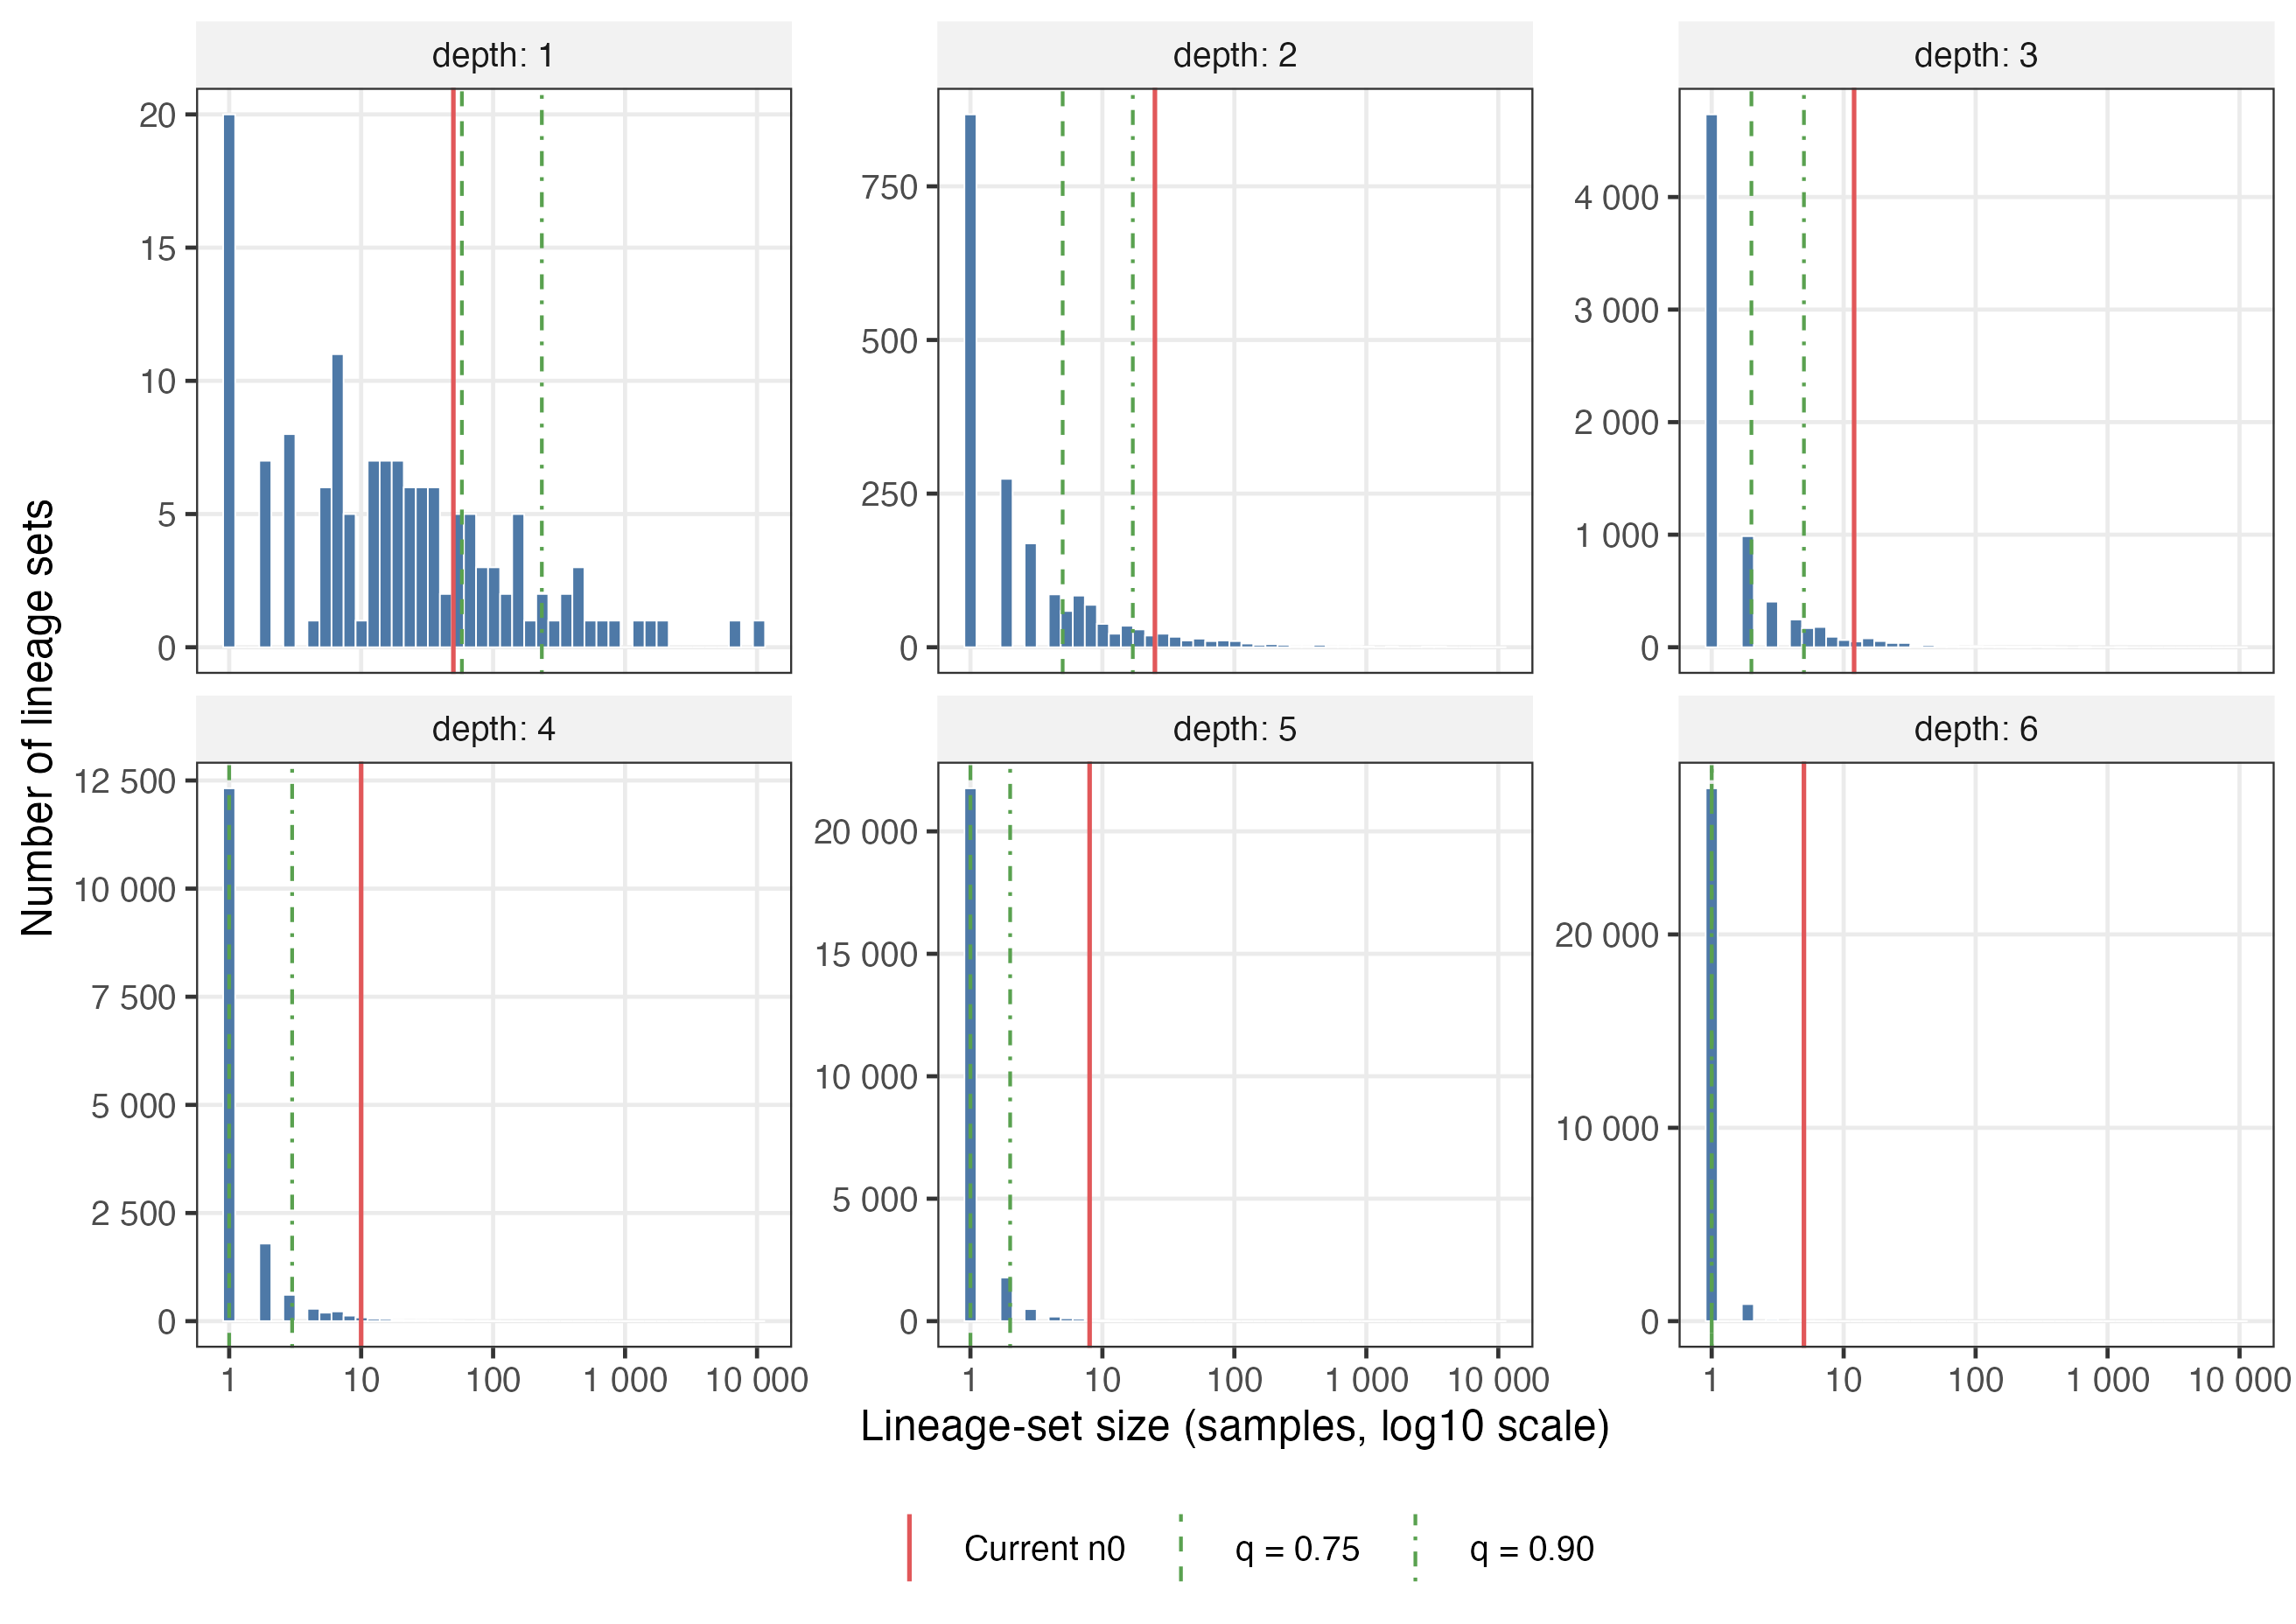
\includegraphics[width=0.98\linewidth]{figures/agp_lineage_size_histograms_depth1_to6.png}
\caption{Histograms of pre-absorption dominance-lineage set sizes for depths 1 through 6. The x-axis is log-scaled because the distributions are strongly right-skewed. Red vertical lines show the current manuscript $n_0$ values; green lines show the 0.75 and 0.90 quantile-derived alternatives.}
\end{figure}

\FloatBarrier
\section*{Quantile-derived candidate schedules}
Table 2 gives candidate $n_0$ schedules from several plausible quantile choices. Lower values of $q$ preserve more named lineages and push less mass into absorption, whereas higher values of $q$ produce a smaller named hierarchy and more aggressive tail absorption. Table 3 gives the corresponding pre-absorption sample share that would lie in lineage sets at or above the candidate threshold, before applying absorb reassignment. Because raw high-depth rank-prefixes are very sparse, high quantiles are included in addition to more conventional central quantiles.

\begin{table}[H]
\centering
\scriptsize
\caption{Candidate $n_0$ values obtained by setting depth-specific $n_0$ to the ceiling of the empirical lineage-set size quantile.}
\resizebox{\linewidth}{!}{\begin{tabular}{lrrrrrr}
\toprule
q & depth\_1 & depth\_2 & depth\_3 & depth\_4 & depth\_5 & depth\_6
 \\
\midrule
0.500 & 15 & 2 & 1 & 1 & 1 & 1
 \\
0.600 & 23 & 2 & 1 & 1 & 1 & 1
 \\
0.700 & 40 & 4 & 2 & 1 & 1 & 1
 \\
0.750 & 58 & 5 & 2 & 1 & 1 & 1
 \\
0.800 & 82 & 6 & 3 & 2 & 1 & 1
 \\
0.900 & 234 & 17 & 5 & 3 & 2 & 1
 \\
0.950 & 588 & 39 & 12 & 5 & 2 & 1
 \\
0.975 & 1449 & 90 & 22 & 8 & 3 & 2
 \\
0.990 & 4913 & 226 & 51 & 15 & 5 & 2
 \\
\bottomrule
\end{tabular}
}
\end{table}

\begin{table}[H]
\centering
\scriptsize
\caption{Pre-absorption sample share in lineage sets retained by each quantile-derived threshold.}
\resizebox{\linewidth}{!}{\begin{tabular}{lrrrrrr}
\toprule
q & depth\_1 & depth\_2 & depth\_3 & depth\_4 & depth\_5 & depth\_6
 \\
\midrule
0.500 & 98.9\% & 97.1\% & 100.0\% & 100.0\% & 100.0\% & 100.0\%
 \\
0.600 & 97.9\% & 97.1\% & 100.0\% & 100.0\% & 100.0\% & 100.0\%
 \\
0.700 & 96.4\% & 93.7\% & 84.4\% & 100.0\% & 100.0\% & 100.0\%
 \\
0.750 & 95.3\% & 92.5\% & 84.4\% & 100.0\% & 100.0\% & 100.0\%
 \\
0.800 & 93.6\% & 91.5\% & 77.9\% & 58.7\% & 100.0\% & 100.0\%
 \\
0.900 & 86.9\% & 84.4\% & 70.6\% & 46.7\% & 26.9\% & 100.0\%
 \\
0.950 & 77.5\% & 76.9\% & 59.2\% & 36.7\% & 26.9\% & 100.0\%
 \\
0.975 & 68.2\% & 67.4\% & 49.6\% & 28.6\% & 14.9\% & 7.3\%
 \\
0.990 & 56.8\% & 53.9\% & 38.5\% & 19.1\% & 7.5\% & 7.3\%
 \\
\bottomrule
\end{tabular}
}
\end{table}

\section*{Interpretation for a methods paper}
The empirical distributions are heavy-tailed at every depth: many lineage sets are small, but a small number of dominant rank-prefixes account for a large fraction of samples. The current manuscript schedule does not behave like one constant unweighted raw-prefix quantile: its empirical percentile is about 71\% at depth 1, about 93--95\% at depths 2 and 3, and above 98\% at depths 4 through 6. A raw-prefix quantile rule is therefore useful as a transparent calibration device, but by itself it becomes too permissive at deep depths unless the selected quantile is very high or an additional minimum floor/refinement rule is imposed.

For manuscript framing, the rule can be stated as follows: for a prespecified quantile $q$, define $n_0(d)=\lceil Q_q\{m_{d1},\ldots,m_{dK_d}\}\rceil$, where $m_{dk}$ is the number of samples in raw depth-$d$ dominance lineage set $k$ after the fixed AGP discovery filters and before absorb reassignment. The absorb-policy hierarchy is then built using the resulting $n_0(1),\ldots,n_0(6)$ schedule. The primary analysis should choose one $q$ before outcome testing; sensitivity analysis should repeat the dCST construction and downstream association summaries over a grid such as $q\in\{0.75,0.90,0.95,0.975,0.99\}$, with an explicit statement if a lower bound on $n_0(d)$ is also imposed at deeper levels.

\section*{Generated files}
\begin{itemize}
\item \texttt{tables/agp\_raw\_lineage\_size\_summary.tsv}: depth-specific distribution summary.
\item \texttt{tables/agp\_quantile\_n0\_candidates.tsv}: long-format quantile threshold table.
\item \texttt{tables/agp\_raw\_lineage\_set\_sizes\_by\_depth.tsv}: all raw lineage-set sizes.
\item \texttt{figures/agp\_lineage\_size\_histograms\_depth1\_to6.png}: combined histogram figure.
\item \texttt{figures/agp\_lineage\_size\_histogram\_depth*.png}: one histogram per depth.
\end{itemize}

\end{document}
